\section{激波与扩展波}

\subsection{激波}

考虑如图\ref{1}所示的导管,可以列写出相关的质量、动量、能量守恒方程式:

\begin{figure}[!ht]
    \centering
    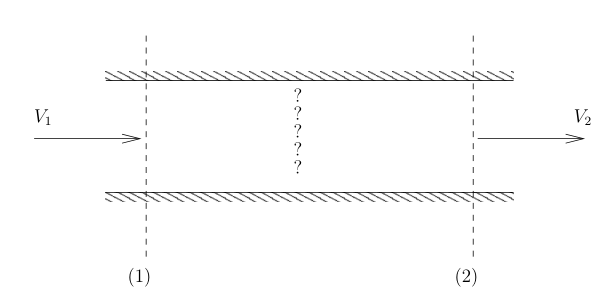
\includegraphics[width=8cm]{figures/1.png}
    \caption{正向激波}
    \label{1}
\end{figure}

\begin{align*}
    \rho_{1} V_{1} A&=\rho_{2} V_{2} A = \dot{m} \\ 
    p_{1} A+\rho_{1} A V_{1}^{2}&=p_{2} A+\rho_{2} A V_{2}^{2}\\ 
    \frac{V_{1}^{2}}{2}+\frac{\gamma}{\gamma-1} \frac{p_{1}}{\rho_{1}}&=\frac{V_{2}^{2}}{2}+\frac{\gamma}{\gamma-1} \frac{p_{2}}{\rho_{2}}
\end{align*}

对于该方程,一个非常直观的解就是$p_1=p_2,\ \rho_1=\rho_2,\ V_1=V_2$.

但除此之外,利用动量式除以质量式,代入能量式,并利用理想气体状态方程,可以得到一个非平凡的解:

\begin{align*}
    \frac{p_{2}}{p_{1}}-1&=\frac{2 \gamma}{\gamma+1}\left(M_{1}^{2}-1\right)\\ 
    \frac{\rho_{2}}{\rho_{1}}-1&=\frac{M_{1}^{2}-1}{1+\frac{\gamma-1}{2} M_{1}^{2}}\\ 
    \frac{T_{2}}{T_{1}}&=\frac{\left(2 \gamma M_{1}^{2}-(\gamma-1)\right)\left(2+(\gamma-1) M_{1}^{2}\right)}{(\gamma+1)^{2} M_{1}^{2}}\\ 
    \frac{T_{2}}{T_{1}}-1&=\frac{2(\gamma-1)\left(\gamma M_{1}^{2}+1\right)\left(M_{1}^{2}-1\right)}{(\gamma+1)^{2} M_{1}^{2}}
\end{align*}

\subsection{导管内的熵变}

\begin{align*}
    Tds&=du+pdv\\ 
    dh&=du+pdv\\ 
    v&=\frac{1}{\rho}\\ 
    ds&=c_p\frac{dT}{T}-R\frac{dp}{p}\\ 
    s_2-s_1&=c_p\ln\left(\frac{T_2}{T_1}\right)-R\ln\left(\frac{p_2}{p_1}\right)=\ln\left[\left(\frac{T_2}{T_1}\right)^{c_p}\left(\frac{p_1}{p_2}\right)^R\right]\\ 
    \frac{s_2-s_1}{c_v}&=\ln\left[\left(\frac{T_2}{T_1}^\gamma\right)\left(\frac{p_1}{p_2}\right)^{\gamma-1}\right]=\ln\left[\left(\frac{\rho_1}{\rho_2}\right)^\gamma\left(\frac{p_2}{p_1}\right)\right]
\end{align*}

代入上一节中关于压力比与密度比的式子,并且定义$m=M_1^2-1$,最终我们可以得到

\begin{equation*}
    \frac{s_{2}-s_{1}}{c_{v}}=\ln \left\{\left[\frac{(m+1)(\gamma-1)+2}{(m+1)(\gamma+1)}\right]^{\gamma}\left[1+\frac{2 \gamma m}{\gamma+1}\right]\right\}=f(m)
\end{equation*}

可以发现,导管内的熵变只与上游马赫数以及绝热指数相关。导管内的熵变可以用两部分来表示,

\begin{equation*}
    s_2-s_1=\Delta s_q+\Delta s_{irr}
\end{equation*}

其中第一项为传热带来的熵变,第二项为不可逆过程带来的熵变。如果考虑绝热流,那么根据热力学第二定律,我们可以得到

\begin{equation*}
    s_2-s_1\geq 0
\end{equation*}

从而

\begin{align*}
    M_1^2-1&\geq 0\\ 
    M_1^2&\geq 0\\ 
    \frac{p_{2}}{p_{1}} \geq 1\\ 
    \frac{\rho_{2}}{\rho_{1}} \geq 1\\ 
    \frac{V_{2}}{V_{1}} \leq 1\\ 
    \frac{T_{2}}{T_{1}} \geq 1\\ 
    \frac{T_{0_{2}}}{T_{0_{1}}}=1
\end{align*}

因此,如果等截面导管内的流体存在熵变,或是流体状态发生改变,那么入口处的流体必须是超音速的。

\subsection{正向激波内的马赫数变化}

仍然从质量守恒(连续性)方程出发,将流速用马赫数替代,并代入理想气体状态方程、声速定义和压力比、密度比关系,可以得到

\begin{align*}
    M_{2}^{2}=\frac{2+(\gamma-1) M_{1}^{2}}{2 \gamma M_{1}^{2}-\gamma+1}\\ 
    M_{2}^{2}-1=\frac{\frac{\gamma+1}{2}\left(1-M_{1}^{2}\right)}{\gamma\left(M_{1}^{2}-1\right)+\frac{\gamma+1}{2}}
\end{align*}

从而,我们得到了出口、入口马赫数$M_2\ M_1$间的关系。如图\ref{2}所示。

\begin{figure}[!ht]
    \centering
    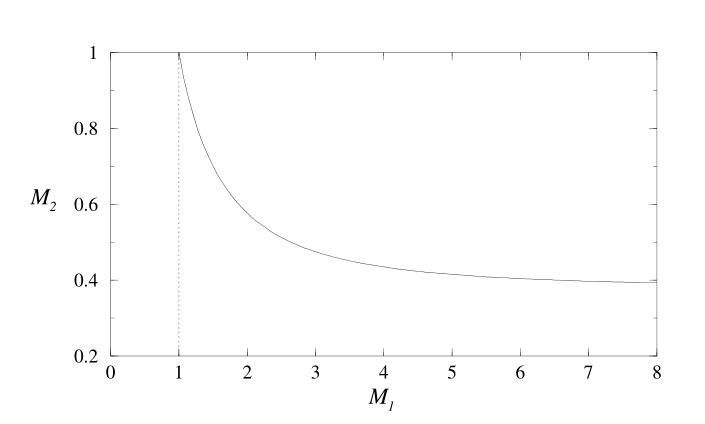
\includegraphics[width=8cm]{figures/2.png}
    \caption{出口、入口马赫数关系}
    \label{2}
\end{figure}

可以看出,入口处为超音速流体,出口处则为亚音速流体。因此可以得出结论:超音速流在经历激波后,变为亚音速流。

\subsection{弱激波下的熵增}

弱激波定义为

\begin{equation*}
    \frac{p_{2}}{p_{1}} \approx 1
\end{equation*}

不难得到,在此条件下的入口马赫数接近$1$。同时由于$m=M_1^2-1\rightarrow0$,因此

\begin{equation*}
    f(m) \approx \frac{1}{15} m^{3}
\end{equation*}

\subsection{滞止压力在激波中的变化}

对于等熵流,我们有

\begin{equation*}
    \frac{p_{0}}{p}=\left(1+\frac{\gamma-1}{2} M^{2}\right)^{\frac{\gamma}{\gamma-1}}
\end{equation*}

但对于激波而言,这个等式并不成立,因为激波本身并不是一个等熵过程。但对于间断面前后的区域,分别有

\begin{align*}
    \frac{p_{0_{1}}}{p_{1}}&=\left(1+\frac{\gamma-1}{2} M_{1}^{2}\right)^{\frac{\gamma}{\gamma-1}}\\ 
    \frac{p_{0_{2}}}{p_{2}}=\left(1+\frac{\gamma-1}{2} M_{2}^{2}\right)^{\frac{\gamma}{\gamma-1}}\\ 
    \frac{p_{0_{2}}}{p_{0_{1}}}=\frac{p_{2}}{p_{1}}\left(\frac{1+\frac{\gamma-1}{2} M_{2}^{2}}{1+\frac{\gamma-1}{2} M_{1}^{2}}\right)^{\frac{\gamma}{\gamma-1}}
\end{align*}

可以替换式中的压力比和$M_2$,从而得到

\begin{equation*}
    \frac{p_{02}}{p_{01}}=\left(\frac{\gamma+1}{2} M_{1}^{2}\right)^{\frac{\gamma}{\gamma-1}}\left(1+\frac{\gamma-1}{2} M_{1}^{2}\right)^{\frac{-\gamma}{\gamma-1}}\left(\frac{2 \gamma}{\gamma+1} M_{1}^{2}-\frac{\gamma-1}{\gamma+1}\right)^{\frac{-1}{\gamma-1}}
\end{equation*}

由于入口处为超音速流,因此$M_1>1$,

\begin{equation*}
    \frac{p_{02}}{p_{01}}<1
\end{equation*}

可以得知,滞止压力在经历激波后将会下降,且入口处马赫数越高,压力下降越多。

\subsection{二维喷管中的流体}

\begin{equation*}
    \frac{A^{*}}{A}=\frac{\left(\frac{p}{p_{o}}\right)^{\frac{1}{\gamma}}\left(1-\left(\frac{p}{p_{o}}\right)^{\frac{\gamma-1}{\gamma}}\right)^{\frac{1}{2}}}{\left(\frac{\gamma-1}{2}\right)^{\frac{1}{2}}\left(\frac{2}{\gamma+1}\right)^{\frac{\gamma+1}{2(\gamma-1)}}}
\end{equation*}

对于一个确定的喷管,如果能够确定出口处流体是超音速流体,那么出口处的压力比$p_e/p_0$就是唯一确定的。但是事实上,出口处的压力可以被设计为任意的值,这会导致在渐扩喷管中一定会出现激波,这个过程会是不可逆的。

\begin{figure}[!ht]
    \centering
    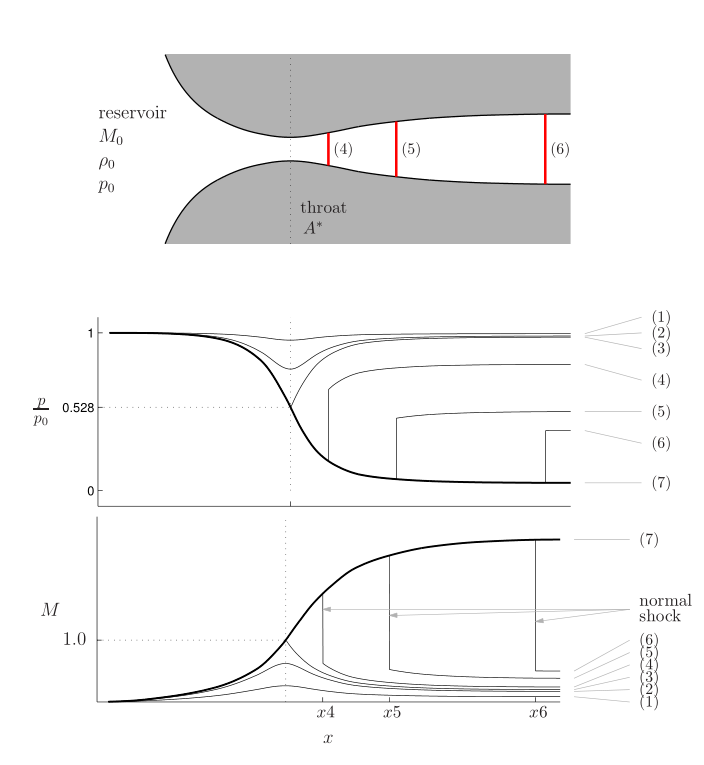
\includegraphics[width=\linewidth]{figures/3.png}
    \caption{出口压力不同导致的激波}
    \label{3}
\end{figure}

如图\ref{3}所示,分别展示了几种不同出口压力下,激波产生的位置。

\begin{itemize}
    \item (7) $p_{e7}/p_0=p_e/p_0$,全过程均为等熵流。
    \item (1),(2) 流体全程均未超过声速,同时全程均为等熵流
    \item (3) 出口压力的设置使得在喉部的流体恰好达到声速。此时,在喉部会发生弱激波,在渐扩喷管部分流体会减速,但流体全程仍为等熵流。
    \item (4) 当$p_{e4}<p_{e3}$时,流体在通过喉部之后将无法保持等熵流,因为出口压力$p_{e4}/p_0>p_{e7}/p_0$,因此一定会在渐扩喷管的某个部分发生激波。
    \item (5),(6) 与(4)类似,但由于压力比与$p_{e7}/p_0$更加接近,因此激波发生的位置也更加接近出口位置
    \item 如果压力进一步降低,斜激波将会发生
\end{itemize}

\subsection{斜激波}

考虑如图\ref{4}所示的斜激波,

\begin{figure}[!ht]
    \centering
    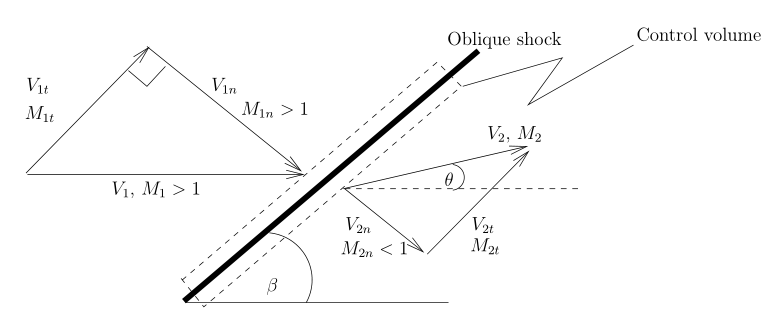
\includegraphics[width=8cm]{figures/4.png}
    \caption{斜激波}
    \label{4}
\end{figure}

考虑连续性方程与切向和法向的动量:

\begin{align*}
    \rho_{1} V_{1 n}&=\rho_{2} V_{2 n}\\ 
    p_{1}+\rho_{1} V_{1 n}^{2}&=p_{2}+\rho_{2} V_{2 n}^{2}\\ 
    \rho_{1} V_{1 n} V_{1 t}&=\rho_{2} V_{2 n} V_{2 t}
\end{align*}

不难得到$V_{1t}=V_{2t}$。由此我们可以得出,对于斜激波,在法向上,其规律与正激波一致;在切向上,速度分量则不产生变化。

如果我们基于上述结果观察一个斜激波,我们就会发现,斜激波的存在会导致流体的流向发生改变,如图\ref{5}所示。

\begin{figure}[!ht]
    \centering
    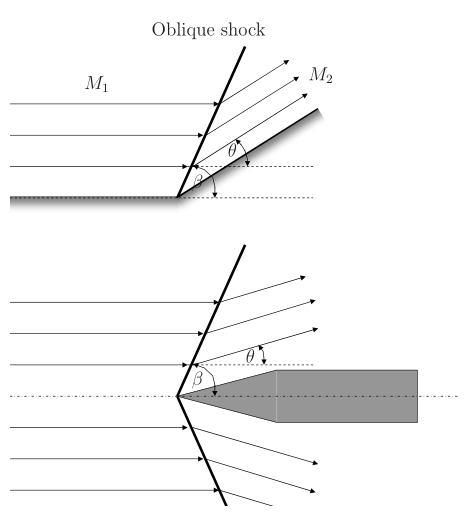
\includegraphics[width=8cm]{figures/5.png}
    \caption{斜激波导致流体流向的变化}
    \label{5}
\end{figure}

\begin{align*}
    M_{1}&=\frac{M_{1 n}}{\sin \beta}\\ 
    M_{2}&=\frac{M_{2 n}}{\sin (\beta-\theta)}
\end{align*}

注意到,$M_1>1$,但$M_{2n}<1$并不意味着$M_2<1$。在经历斜激波后,流体仍然可能是超音速的。

\subsection{马赫角}

对于超音速流体,如图\ref{6}所示的圆锥顶角称为马赫角$\mu$,

\begin{figure}[!ht]
    \centering
    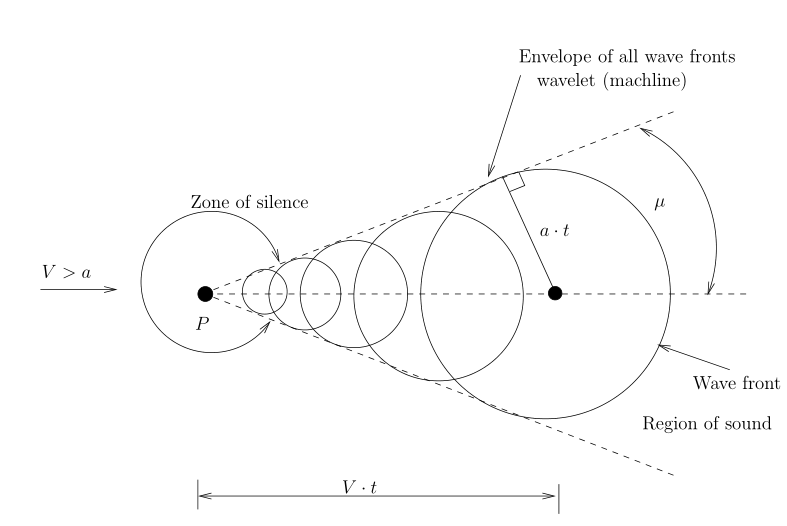
\includegraphics[width=8cm]{figures/6.png}
    \caption{马赫角}
    \label{6}
\end{figure}

满足

\begin{align*}
    \sim\mu&=\frac{a}{V}=\frac{1}{M}\\ 
    M&=\frac{1}{\sin\mu}\\ 
    \sin\mu&=\frac{1}{M}
\end{align*}

当超音速流体遇到遇到较强的物理约束时,此时斜激波就会产生,并且满足关系

\begin{equation*}
    M_{1 n}=M_{1} \sin \beta=\frac{\sin \beta}{\sin \mu}>1
\end{equation*}

斜激波的角度始终大于马赫角,$\beta>\mu$。

\subsection{偏折角$\theta$与激波倾角$\beta$间的关系}

\begin{figure}[!ht]
    \centering
    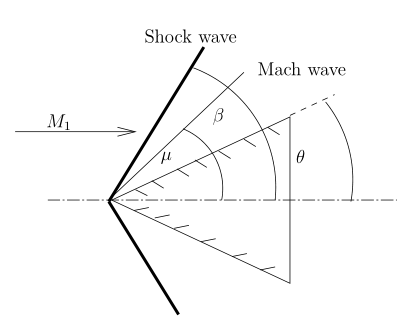
\includegraphics[width=8cm]{figures/7.png}
    \caption{偏折角与激波倾角间的关系}
    \label{7}
\end{figure}

利用之前的结论,对于斜激波,在法向上,正激波的结论依然适用,因此

\begin{equation*}
    \frac{\rho_{2}}{\rho_{1}}=\frac{\frac{\gamma+1}{2}\left(M_{1} \sin \beta\right)^{2}}{1+\frac{\gamma-1}{2}\left(M_{1} \sin \beta\right)^{2}}
\end{equation*}

考虑到激波两侧的连续性,因此

\begin{align*}
    \frac{\rho_{2}}{\rho_{1}}&=\frac{V_{1 n}}{V_{2 n}}\\ 
    &=\frac{V_{1 n}}{V_{1 t}} \frac{V_{2 t}}{V_{2 n}}\\ 
    &=\frac{\tan \beta}{\tan (\beta-\theta)}
\end{align*}

把上述两式进行比较,可以得到

\begin{align*}
    \tan \theta&=\frac{\tan \beta\left(M_{1}^{2} \sin ^{2} \beta-1\right)}{\tan ^{2} \beta \frac{\gamma}{2} M_{1}^{2}+\frac{1}{2} M_{1}^{2} \sin ^{2} \beta\left(1-\tan ^{2} \beta\right)+\tan ^{2} \beta}\\ 
    &=2 \cot \beta\left[\frac{M_{1}^{2} \sin ^{2} \beta-1}{M_{1}^{2}(\gamma+\cos 2 \beta)+2}\right]
\end{align*}

对应关系可以从图\ref{8}中得到更直观的了解。

\begin{figure}[!ht]
    \centering
    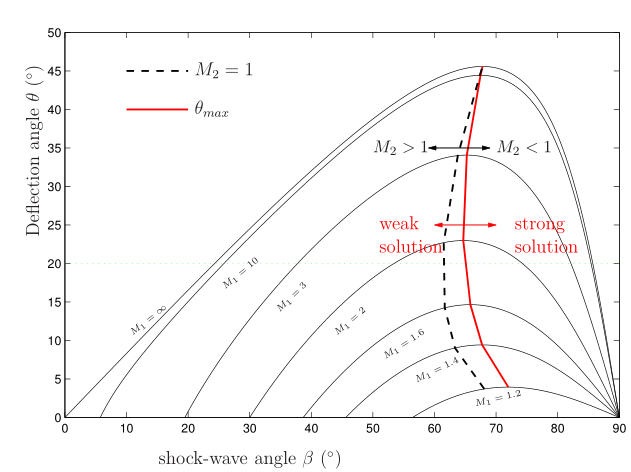
\includegraphics[width=8cm]{figures/8.png}
    \caption{$\theta$ vs. $\beta$}
    \label{8}
\end{figure}

可以看出,对于给定的$\theta$角,有两个$\beta$角与之对应,其中一个为出流马赫数小于1的强解,另一个为出流马赫数大于1的弱解。在实际中,出现的究竟是强解还是弱解,取决于背景中的压力;一般而言,弱解更加常见,但是如果提升背景压力,则强解也有可能出现。

\begin{align*}
    M_{2 \text { strong }}&<M_{2 \text { weak }}\\ 
    \beta_{\text {strong }}&>\beta_{\text {weak }}
\end{align*}

\subsection{斜激波的特殊解}

\begin{enumerate}
    \item 从喷管进入高压区域的超音速流体(喷气式飞机)
    
    当$p_{e7}<p_e<p_{e6}$时,接近出口处的流体将会是超音速流,并且在喷管出口处的压力将会与$p_{e7}$相等,但当流体到达出口处时,必须立刻提升压力到$p_e$,为了达到这样的效果,斜激波会在出口的边角处生成。

    涡流层的存在是压力发生骤变的原因。把正激波的式子代入斜激波的法向,可以得到

    \begin{equation*}
        \frac{p_{2}}{p_{1}}=\frac{2 \gamma}{\gamma+1}\left(M_{1}^{2} \sin ^{2} \beta-1\right)
    \end{equation*}

    其中$p_1$是出口前压力,$p_2$是出口后压力,通过这个式子以及已知的$M_1$,我们可以得到对应的$\beta$角,从而找到对应的$\theta$和$M_2$。

    \item 固体边界带来的激波反射
    
    当激波碰到墙时,激波也会反射,而对应的反射角由墙带来的边界条件确定:原本平行于墙面的流体在经过激波的两次折射后,仍然平行于墙面,如图\ref{9}所示。

    \begin{figure}[!ht]
        \centering
        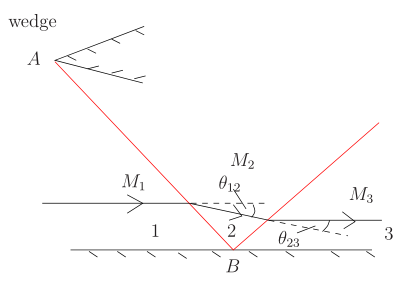
\includegraphics[width=8cm]{figures/9.png}
        \caption{激波的反射}
        \label{9}
    \end{figure}
\end{enumerate}

\subsection{马赫线与其性质}

